%
% standardmodell.tex -- slide template
%
% (c) 2021 Prof Dr Andreas Müller, OST Ostschweizer Fachhochschule
%
\bgroup
\begin{frame}[t]
\setlength{\abovedisplayskip}{5pt}
\setlength{\belowdisplayskip}{5pt}
\frametitle{Standardmodell}
\vspace{-20pt}
\begin{columns}[t,onlytextwidth]
\begin{column}{0.53\textwidth}
%\vspace{-18pt}
\begin{center}
\only<1>{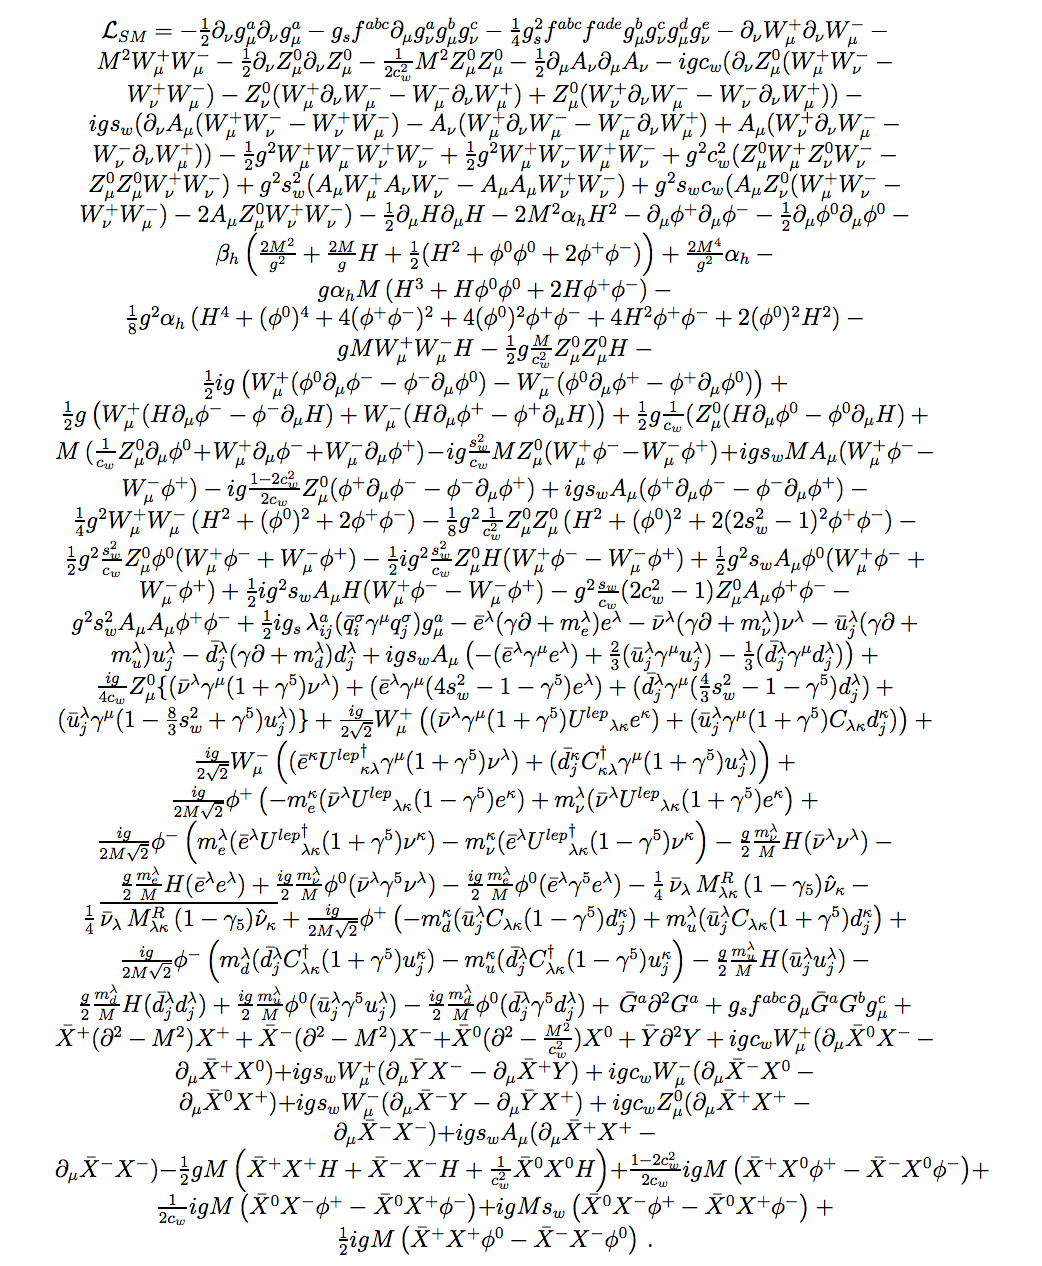
\includegraphics[width=\textwidth]{../slides/4/sm.png}}%
\only<2->{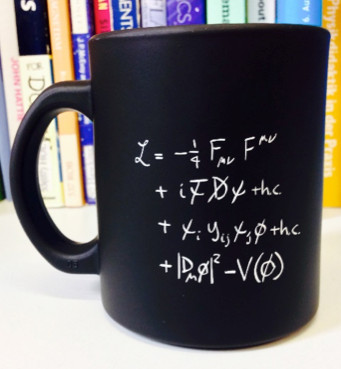
\includegraphics[width=\textwidth]{../slides/4/smtasse.jpg}}%
\end{center}
\end{column}
\begin{column}{0.43\textwidth}
\uncover<3->{%
\begin{block}{Lagrange-Dichte für alle Felder\strut}
\begin{center}
\renewcommand\arraystretch{1.3}
\begin{tabular}{rp{4cm}}
\text{Feld}&Teilchen\\
\hline
\uncover<4->{$F_{\mu\nu}$ &Bosonen-Felder: Photonen, $W$- und $Z$-Bosonen, Gluonen}\\
\uncover<5->{$\psi$       &Fermionen-Felder: Quarks, Leptonen, Neutrions}\\
\uncover<6->{$\phi$       &Higgs-Bosonen}
\end{tabular}
\end{center}
\uncover<7->{Alle Teilchen/Wechselwirkungen ausser die Gravitation}
\end{block}}
\end{column}
\end{columns}
\end{frame}
\egroup
